\documentclass[14pt,xcolor=dvipsnames]{beamer}
\usetheme{AnnArbor}
\usecolortheme{crane}

\usepackage{hyperref}   
\usepackage{url}
\hypersetup{urlcolor=red}

\renewcommand{\bibname}{References}
\setbeamertemplate{bibliography item}{[\theenumiv]}

\usepackage{kbordermatrix}
\usepackage{multicol}
\usepackage{verbatim} 
\usepackage{graphics}
\usepackage{graphicx}
\usepackage{tikz}


%Basic Information
\title{Graph Based Storage for Relational Database}
\author{Adarsh, Ajith, Ashish, Sourabh}
\date{\today}

%--------------------------------------------------------------------------------------
%               TITLE PAGE (Slide 1)
%--------------------------------------------------------------------------------------
\begin{document}
\begin{frame}
\titlepage
\end{frame}
%--------------------------------------------------------------------------------------


%--------------------------------------------------------------------------------------
%               Outline
%--------------------------------------------------------------------------------------
\begin{frame}
\frametitle{Outline}
\begin{multicols}{2}
\tableofcontents[hideallsubsections]
\end{multicols}
\end{frame}

\section{Introduction}
\begin{frame}
\frametitle{Introduction}
\begin{itemize} 
 \item Problem Description
  \begin{itemize}
    \item Data redundancy
    \item Join query
  \end{itemize}
\end{itemize}
\end{frame}

\section{Problem Statement}
\begin{frame}
\frametitle{Problem Statement}
\begin{itemize}
  \item To develop a data storage system based on graph structure in order to optimize the query execution time especially join queries and eliminate some sort of data redundancy in a relational model while retaining other advantages of relational database system in terms of performance of other queries.
\end{itemize}
\end{frame}

\section{Objectives}
\begin{frame}
 \frametitle{Objectives}
 \begin{itemize}
 \item<1-> To explore the pros and cons of the graph model.
 \item<2-> To compare the relational model with the graph model.
 \item<3-> To develop a model which can represent relational database.
 \item<4-> To define relational algebraic operations on the model such that it has most of the advantages of both the models.
 \item<5-> To understand the differences of the proposed model with the graph model.
 \item<6-> To realize the limitations of the proposed model.
 \end{itemize}
\end{frame}

\section{Overview of Model}
\begin{frame}
 \frametitle{Overview of the Model}
 \begin{itemize}
  \item<1-> A database consist of multiple tables
  \item<2-> Each table is a collection of domains
  \item<3-> Each table contains list of main node records
 \end{itemize}
\end{frame}

\begin{frame}
\begin{figure}[t]
 \centering
 \includegraphics[width=0.7\textwidth]{pics/model.pdf}
 \caption{Overview of Proposed Graph Based Storage}
 \label{fig:overview}
\end{figure}
\end{frame}

\begin{frame}
 \frametitle{Overview of the Model}
 \begin{itemize}
  \item<1-> A database consist of multiple tables
  \item<1-> Each table is a collection of domains
  \item<1-> Each table contains list of main node records
  \item<2-> Each Domain is collection of attribute nodes
  \item<3-> Each attribute node contains the actual data elements
 \end{itemize}
\end{frame}

\section{Handling Constraints}
\begin{frame}
 \frametitle{Handling Constraints}
 \begin{itemize}
  \item Primary Key
 \end{itemize}
\end{frame}

\begin{frame}
 \frametitle{Primary Key}
 \begin{figure}
 \centering
 \includegraphics[width=0.7\textwidth]{pics/primary_key.pdf}
 \caption{Primary Keys in Proposed Model}
 \label{fig:primary_key}
\end{figure}
\end{frame}

\begin{frame}
 \frametitle{Handling Constraints}
 \begin{itemize}
  \item Primary Key
  \item Foreign Key
 \end{itemize}
 \end{frame}

\begin{frame}
 \frametitle{Foreign Key}
 \begin{figure}[h]
 \centering
 \includegraphics[width=0.45\textwidth]{pics/foreign_key.pdf}
\end{figure}
\end{frame}

\begin{frame}
 \frametitle{Handling Constraints}
 \begin{itemize}
  \item Primary Key
  \item Foreign Key
  \item Other Foreign Key Models
  \begin{itemize}
    \item<2-> Direct Connection Model
    \item<3-> Shared Domain Model
    \item<4-> Duplicate Domain Model
  \end{itemize}
 \end{itemize}
\end{frame}
 
\section{Indexing}
\begin{frame}
 \frametitle{Indexing Using Trie}
 \begin{figure}
 \centering
 \includegraphics[width=0.5\textwidth]{pics/trie.pdf}
 \caption{Trie Data Structure for Indexing}
 \end{figure}
\end{frame}

\section{Query Handling}
\begin{frame}
\frametitle{Insert Query}
\begin{itemize}
 \item<1-> Check for constraints (Primary and Foreign Key)
 \item<2-> Find or Create attribute nodes with given value
 \item<3-> Create main node and add to main list
 \item<4-> Connect main node with attribute nodes
\end{itemize}
\end{frame}

\begin{frame}
 \frametitle{Select Query}
 \begin{itemize}
  \item<1-> Find attribute nodes satisfying given propositional formula
  \item<2-> Get list of corresponding main nodes
  \item<3-> Perform Union or Intersection as required
  \item<4-> Project on the resultant set of records
  \item<5-> Print the result
 \end{itemize}
\end{frame}

\begin{frame}
 \frametitle{Update and Delete Query}
 \begin{itemize}
  \item<1-> Select records according to given conditions
  \item<2-> Find corresponding attribute nodes
  \item<3-> Create or find attribute nodes with the updated values if required
  \item<4-> Connect or disconnect main node with attribute nodes if required
  \item<5-> Mark main node for soft delete if required
 \end{itemize}
\end{frame}

\begin{frame}
 \frametitle{Join Query}
 \begin{itemize}
  \item<1-> Select records in parent relation satisfying propositional formula
  \item<2-> Get list of main nodes in child relation corresponding to filtered parent records
  \item<3-> Select records in child relation satisfying propositional formula
  \item<4-> Perform intersection or union as required
  \item<5-> Project on the resultant set of records
  \item<6-> Print the result
 \end{itemize}
\end{frame}

\section{Results \& Analysis}
\begin{frame}
 \frametitle{Results \& Analysis}
 \begin{itemize}
  \item Size Measurement
 \end{itemize}
\end{frame}

\begin{frame}
 \frametitle{Size Measurement}
 \begin{figure}
 \centering
 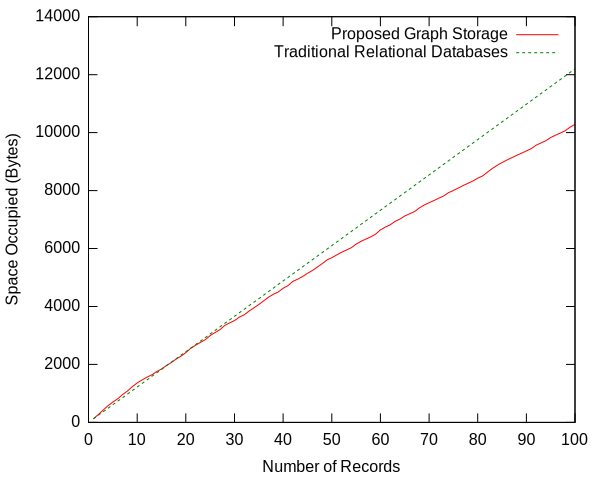
\includegraphics[width=0.8\textwidth]{pics/100.pdf}
 \end{figure}
\end{frame}

\begin{frame}
 \frametitle{Results \& Analysis}
 \begin{itemize}
  \item Size Measurement
  \item Time Measurement
 \end{itemize}
\end{frame}

\begin{frame}
 \frametitle{Time Measurement}
 \begin{figure}
 \centering
 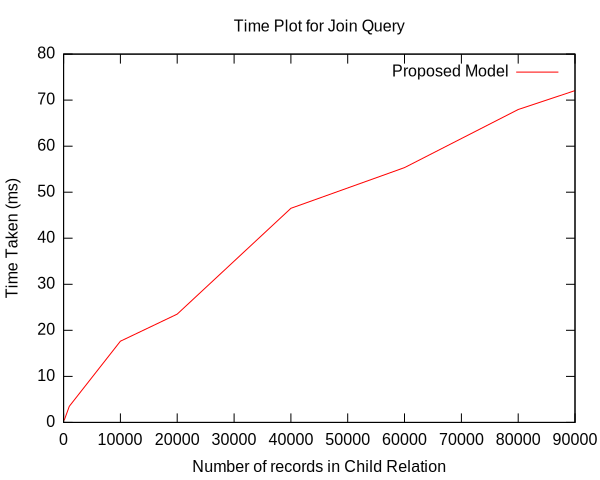
\includegraphics[width=0.7\textwidth]{pics/time.pdf}
 \end{figure}
\end{frame}

\begin{frame}
\frametitle{Thank You}
 \huge
 \centering
 \vspace{1cm}
 Thank You ! \\
 \vspace{1.5cm}
 \flushright 
 \flushbottom
 \small
 Adarsh Mohata - 12IT03 \\
 Ajith P S - 12IT04\\
 Ashish Kedia - 12IT14 \\
 Sourabh Suman - 12IT82
\end{frame}

\end{document}